\chapter{Méthodes de Rétrécissement (Shrinkage Methods)}
\section{Introduction aux Méthodes de Rétrécissement (Shrinkage Methods)}

Les méthodes traditionnelles de sélection de sous-ensembles utilisent les moindres carrés pour ajuster un modèle linéaire contenant un sous-ensemble des prédicteurs. 
En alternative, nous pouvons ajuster un modèle contenant l'ensemble des $p$ prédicteurs en utilisant une technique qui contraint ou régularise les estimations des coefficients. 
De manière équivalente, cela rétrécit (shrink) les estimations des coefficients vers zéro. 
Il n'est pas forcément évident de comprendre pourquoi une telle contrainte améliore l'ajustement, mais il s'avère que le rétrécissement des coefficients permet de réduire significativement leur variance.

\subsection{Précision de Prédiction et Erreur Quadratique Moyenne (MSE)}

Supposons que nous observons des données de la forme :
$$y_i = f(x_i) + \epsilon_i, \quad i=1,...,n$$ 
où $f : \mathbb{R}^p \rightarrow \mathbb{R}$. 
Les $x_i \in \mathbb{R}^p$ sont des mesures de prédicteurs fixes. 
Les $\epsilon_i \in \mathbb{R}$ sont des erreurs aléatoires avec $\mathbb{E}(\epsilon_i) = 0$, $Var(\epsilon_i) = \sigma^2$ et $Cov(\epsilon_i, \epsilon_j) = 0$.

Considérons un nouveau point de donnée $y_0 = f(x_0) + \epsilon_0$, indépendant des précédents, que nous cherchons à prédire à l'aide de $\hat{f}(x_0)$. 
L'erreur de prédiction (PE) est liée à l'erreur quadratique moyenne (MSE) par la relation suivante :
$$PE(\hat{f}(x_0)) = \mathbb{E}[(y_0 - \hat{f}(x_0))^2]$$ 
$$PE(\hat{f}(x_0)) = \sigma^2 + MSE(\hat{f}(x_0))$$ 
Ainsi, le PE et le MSE représentent essentiellement le même concept : optimiser l'un revient à optimiser l'autre.

\subsection{Décomposition Biais-Variance}

L'erreur quadratique moyenne (MSE) dépend de deux quantités fondamentales :
$$MSE(\hat{f}(x_0)) = \text{Biais}(\hat{f}(x_0))^2 + Var(\hat{f}(x_0))$$ 
Ceci est connu sous le nom de compromis biais-variance.

\begin{figure}[h]
    \centering
    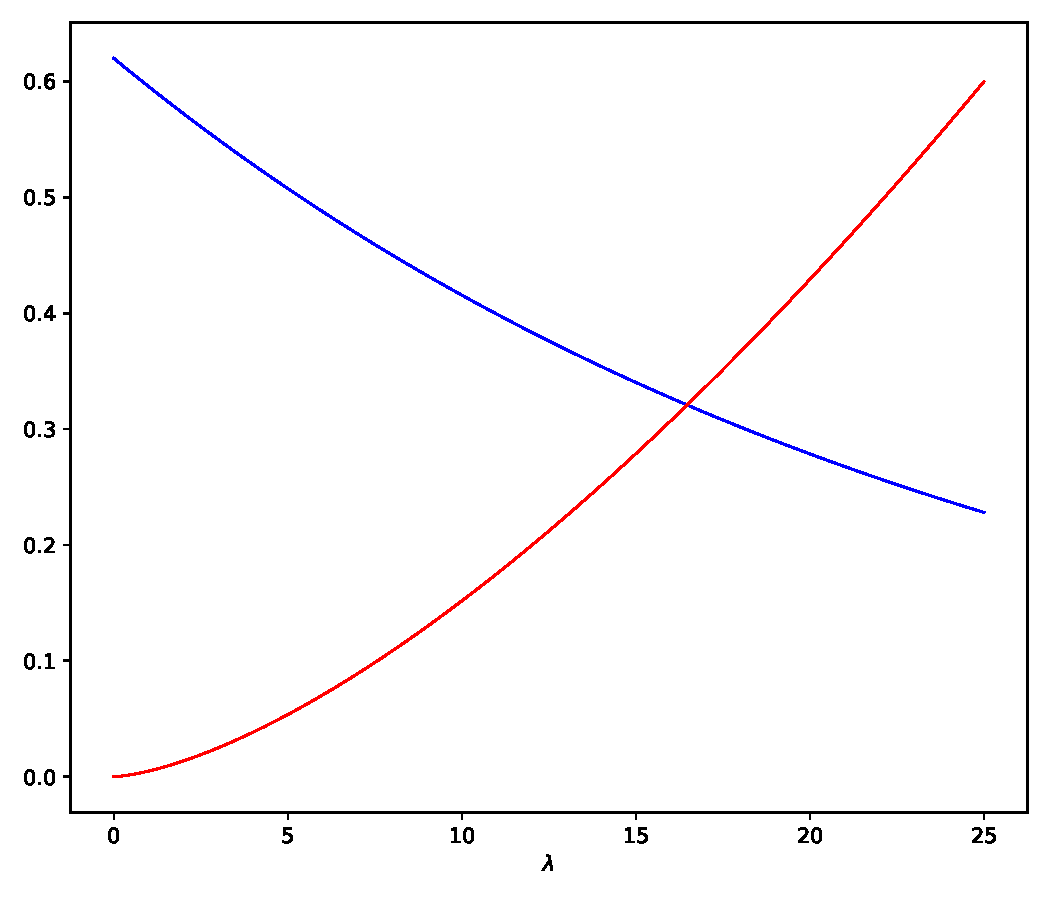
\includegraphics[width=0.6\textwidth]{images/bias_var.pdf}
    \caption{Évolution du Biais au carré (en rouge) et de la Variance (en bleu) en fonction de la flexibilité ou de la pénalité ($\lambda$).}
    \label{fig:bias_var}
\end{figure}

\subsection{Modèle Linéaire et Théorème de Gauss-Markov}

Dans le cadre d'un modèle linéaire, on suppose $f(x_i) = x_i^T \beta^*$. 
La prédiction par les moindres carrés (LS) est donnée par $\hat{f}^{LS}(x_i) = x_i^T \hat{\beta}$. 
Le théorème de Gauss-Markov stipule que cet estimateur est le "BLUE" (Best Linear Unbiased Estimator). 
Cela signifie que parmi tous les estimateurs linéaires et sans biais, l'estimateur des moindres carrés possède la plus petite variance, et donc le plus petit MSE.

Cependant, il est possible de construire un autre estimateur linéaire (qui introduit un biais) mais qui possède un MSE global inférieur à celui de l'estimateur des moindres carrés.

En analysant l'erreur pour la régression linéaire sur l'ensemble des points, on obtient :
$$PE(\hat{f}) = \sigma^2 + 0 + \frac{p\sigma^2}{n}$$ 
La variance $\frac{1}{n} \sum Var(x_i^T \hat{\beta})$ correspond exactement à $\frac{p\sigma^2}{n}$. 
Cela démontre que la variance croît linéairement avec le nombre de prédicteurs $p$. 
Chaque variable prédictive supplémentaire ajoute la même quantité de variance $\frac{\sigma^2}{n}$, que son vrai coefficient soit grand, petit ou nul. 
Nous pouvons donc faire mieux en rétrécissant (shrink) les petits coefficients vers zéro. 
Cela introduit un biais, mais réduit considérablement la variance pour obtenir une image globale plus stable.

\section{Régression Ridge}

\subsection{Formulation du Modèle}

La procédure des moindres carrés (LS) estime les coefficients en minimisant le RSS :
$$RSS = \sum_{i=1}^{n} \left( y_i - \beta_0 - \sum_{j=1}^{p} \beta_j x_{ij} \right)^2$$ 
En contraste, la régression Ridge estime les coefficients $\hat{\beta}^R$ en minimisant la quantité suivante :
$$RSS + \lambda \sum_{j=1}^{p} \beta_j^2$$ 
où $\lambda \ge 0$ est un paramètre de réglage qui contrôle la force du terme de pénalité.
\begin{itemize}
    \item Lorsque $\lambda = 0$, on retrouve l'estimation de la régression linéaire classique.
    \item Lorsque $\lambda = \infty$, la pénalité force les coefficients à être nuls : $\hat{\beta}^R = 0$.
\end{itemize}
Le second terme est une "pénalité de rétrécissement" qui pousse les estimations des $\beta_j$ vers zéro. 
Le choix d'un bon paramètre $\lambda$ est critique et se fait généralement par validation croisée.

\begin{figure}[h]
    \centering
    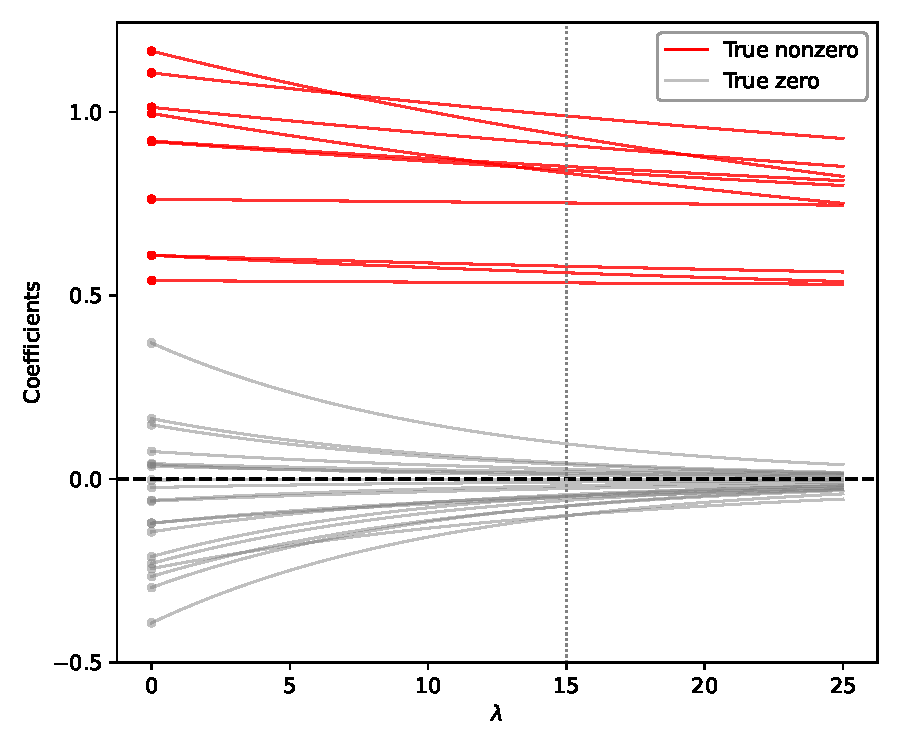
\includegraphics[width=0.8\textwidth]{images/ridge_coef_paths.pdf}
    \caption{Shrinkage des coefficients de la régression Ridge en fonction de $\lambda$. Les coefficients convergent asymptotiquement vers 0 sans jamais l'atteindre exactement.}
    \label{fig:ridge_coef_paths}
\end{figure}

\subsection{Solution Analytique}

En calculant la dérivée du critère $(y - X\beta)^T(y - X\beta) + \lambda \beta^T \beta$ par rapport à $\beta$, on obtient les équations normales de Ridge:
$$X^T y = (X^T X + \lambda I_p)\beta$$ 
Ce qui donne l'estimateur Ridge explicite :
$$\hat{\beta}^R = (X^T X + \lambda I_p)^{-1} X^T y$$ 
Contrairement à l'estimateur des moindres carrés qui n'existe pas toujours (si $X^T X$ n'est pas inversible), la solution Ridge est toujours unique pour $\lambda > 0$, car la matrice $(X^T X + \lambda I_p)$ est toujours inversible.

\textbf{($\bigstar$ EXAMEN) Prédicteurs identiques (Grouping Effect) :} Si deux variables sont rigoureusement identiques temporellement (ex: $n=2, p=2, X_1 = X_2$), la régression Ridge divisera exactement les coefficients de manière égale ($\hat{\beta}_1^R = \hat{\beta}_2^R$). Le Lasso, au contraire, est mathématiquement instable dans cette configuration et choisira arbitrairement l'une des deux variables en annulant le coefficient de l'autre.

\subsection{Mise à l'échelle des Prédicteurs (Scaling)}

Les estimateurs des moindres carrés sont invariants à l'échelle : multiplier un prédicteur $X_j$ par une constante $c$ entraîne simplement la division du coefficient estimé par $c$, gardant $X_j \hat{\beta}_j$ inchangé. 
À l'inverse, les estimations de la régression Ridge peuvent changer substantiellement si l'on multiplie un prédicteur par une constante. 
Ceci est dû à la somme des carrés des coefficients dans la pénalité. 
Il est donc \textbf{absolument impératif de centrer-réduire (standardiser)} les prédicteurs avant d'ajuster un modèle Ridge ou Lasso, sous peine d'attribuer par erreur une faible pénalité aux variables possédant des valeurs modélisées sur une grande échelle unitaire.

\textbf{($\bigstar$ EXAMEN) Règle d'Or (Validation et Test) :} Lors de l'évaluation sur un jeu de test, il faut \textbf{impérativement utiliser la moyenne et l'écart-type calculés sur l'ensemble d'entraînement} pour standardiser les données de test. Jamais l'inverse, sous peine de fuite de données (data leakage). Par exemple, si l'intervalle d'entraînement était $[-10, 10]$ et qu'on l'a ramené à $[-1, 1]$ (soit une division par $10$), des valeurs test évoluant sur $[-11, 8]$ devront impérativement devenir $[-1.1, 0.8]$, de façon purement proportionnelle.

\subsection{Forme Contrainte et Géométrie}

La régression Ridge peut être reformulée comme un problème d'optimisation sous contrainte :
$$\hat{\beta}^R = \arg\min_{\beta \in \mathbb{R}^p} ||y - X\beta||_2^2 \quad \text{s.c.} \quad ||\beta||_2^2 \le s$$ 
Géométriquement, la contrainte Ridge (pénalité $L_2$) définit une région en forme de cercle (ou hypersphère) centrée sur l'origine. 
Les estimations Ridge sont données par le premier point de contact entre les ellipses d'isovaleurs du RSS (centrées sur $\hat{\beta}^{LS}$) et cette région de contrainte ronde. En raison de l'absence de "coins", les ellipses touchent presque toujours la frontière du cercle sans intercepter exactement un axe. De ce fait, les coefficients Ridge contournent le zéro (ils rétrécissent asymptotiquement) sans jamais s'y annuler formellement.

\subsection{Lien entre Moindres Carrés et Ridge (Opérateur Linéaire)}

En posant l'opérateur linéaire matriciel $W = (X^T X + \lambda I_p)^{-1} X^T X$, on trouve une relation analytique fondamentale liant l'estimateur Ridge à celui des moindres carrés (OLS) via une simple transformation géométrique :
\textbf{($\bigstar$ EXAMEN)}
\begin{equation}
\hat{\beta}^{Ridge} = W \hat{\beta}^{LS}
\end{equation}
De ce fait, la variance de l'estimateur Ridge se formule formellement en fonction de la matrice de covariance originelle $(X^T X)^{-1}$ :
\textbf{($\bigstar$ EXAMEN)}
\begin{equation}
\mathbb{V}[\hat{\beta}^{Ridge}] = \sigma^2 W (X^T X)^{-1} W^T
\end{equation}
On a toujours $\mathbb{V}(x^T \hat{\beta}^{LS}) \ge \mathbb{V}(x^T \hat{\beta}^{Ridge})$. 

\textbf{($\bigstar$ EXAMEN) Cas particulier Orthonormal ($X^T X = I_p$) :} 
Si les variables explicatives sont orthonormales, la relation se simplifie considérablement en $\hat{\beta}^{Ridge} = \frac{1}{1+\lambda} \hat{\beta}^{LS}$, ce qui nous permet de dériver directement l'Espérance et la Variance du nouvel estimateur :
\begin{equation}
\mathbb{E}[\hat{\beta}^{Ridge}] = \frac{1}{1+\lambda} \beta
\end{equation}
\begin{equation}
\mathbb{V}[\hat{\beta}^{Ridge}] = \frac{\sigma^2}{(1+\lambda)^2} I_p
\end{equation}
L'erreur quadratique moyenne de l'estimateur Ridge (somme intégrale de la variance et du biais scalaire au carré) devient alors explicitement :
\begin{equation}
MSE(\hat{\beta}^R) = (1+\lambda)^{-2}(p\sigma^2 + \lambda^2 \beta^T \beta)
\end{equation}
\end{equation}
Le biais augmente avec $\lambda$, tandis que la variance calculée sur les données de test va \textbf{diminuer de façon monotone} (\textit{steadily decrease}). Un compromis est donc nécessaire pour optimiser le MSE.

\textbf{($\bigstar$ EXAMEN) Raisonnement Type - Flexibilité et Biais-Variance} : 
Il est essentiel de formuler l'arbitrage ainsi : \textit{"Comparé aux moindres carrés, Ridge (ou tout estimateur régularisé) est \textbf{moins flexible} (il contraint les coefficients). Par conséquent, il \textbf{améliore la précision des prédictions} lorsque la baisse de sa \textbf{variance} excède largement la légère augmentation de son \textbf{biais}."} 

\textit{Sens de variation} : Attention au sens du paramètre ! Si l'on écrit la contrainte de norme comme $\sum |\beta_j| \le s$ (ou $||\beta||_2^2 \le s$), alors \textbf{quand $s$ augmente, la flexibilité augmente} (on "relâche" le corset vers la solution libre des moindres carrés). En conséquence, la variance augmente et le biais diminue, dessinant une courbe en "U" classique pour l'erreur de test globale.

\begin{figure}[h]
    \centering
    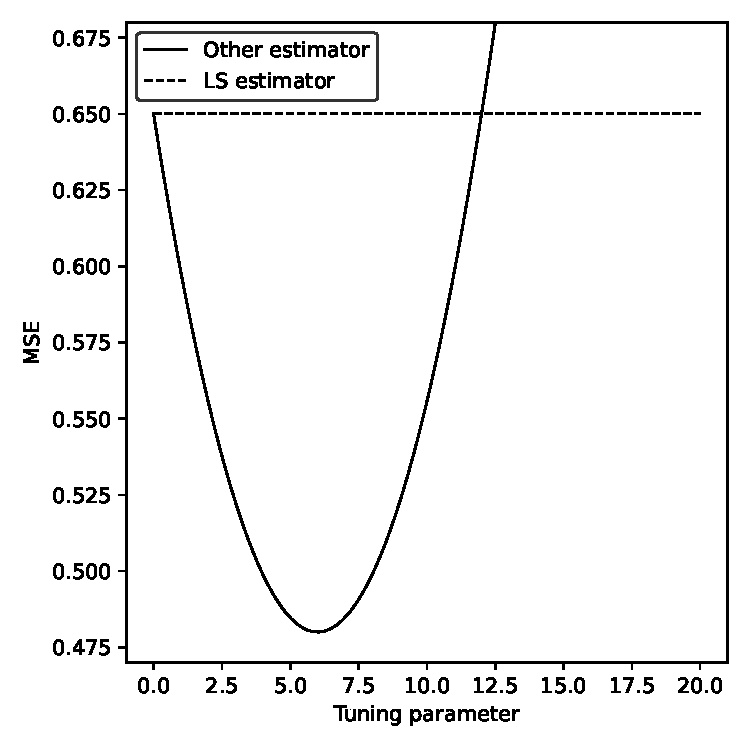
\includegraphics[width=0.5\textwidth]{images/ridge_mse_simple.pdf}
    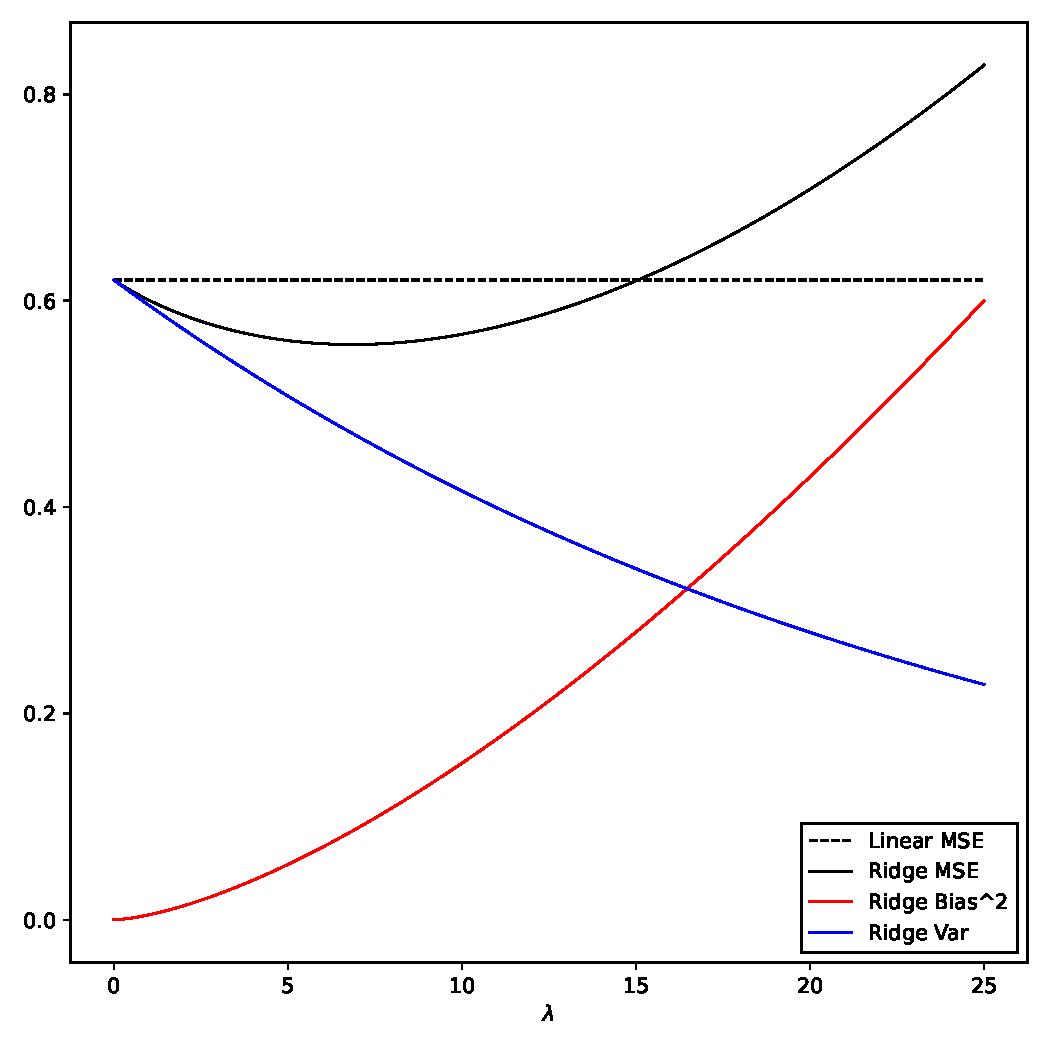
\includegraphics[width=0.45\textwidth]{images/ridge_mse_decomposition.pdf}
    \caption{Compromis Biais-Variance : Évolution de l'erreur quadratique moyenne (MSE) de l'estimateur Ridge en fonction du paramètre de pénalité $\lambda$. L'estimateur robuste permet de dépasser les moindres carrés.}
    \label{fig:ridge_mse}
\end{figure}

\section{Applications en Traitement d'Image : Pénalisation}

\subsection{Données Manquantes et Inpainting}
Dans de nombreuses situations en traitement d'images, des pixels peuvent manquer (défaut de capteur, compression, altération). 
Restaurer ces parties manquantes est appelé "inpainting".

Le modèle de dégradation entre l'image parfaite $x$ et l'image observée dégradée $s$ s'écrit :
$$s = Hx$$ 
où $H$ est une matrice diagonale valant 1 si le pixel est observé, et 0 sinon. 
Estimer $x$ à partir de $s$ est un problème inverse mal posé car il y a moins d'observations que d'inconnues.

\subsection{Régularisation de Tikhonov (Ridge en image)}
Pour stabiliser l'inversion, on impose que l'énergie des variations de l'image soit faible. On minimise la fonctionnelle suivante :
$$J(x) = \underbrace{\frac{1}{2} ||s - Hx||^2}_{\text{Fidélité aux données}} + \underbrace{\frac{\lambda}{2} ||\Delta x||^2}_{\text{Pénalité}}$$ 
La convexité de $J$ implique l'existence d'un minimum global. 
La dérivée du terme d'attache aux données $\frac{1}{2} ||s - Hx||^2$ est formellement $-H^T(s - Hx)$. Or, puisque $H$ est un masque diagonal binaire ($H^T = H$ et $H^2 = H$) et que les observations manquantes dans $s$ valent 0 ($Hs = s$), on a $H^T(s - Hx) = s - Hx$.
La solution peut donc être trouvée via une méthode de descente de gradient à pas fixe très optimisée :
$$x^{(t+1)} = x^{(t)} + \mu (s - Hx^{(t)} - \lambda \Delta^* \Delta x^{(t)})$$ 
La condition de convergence pour le pas $\mu$ est $0 < \mu < \frac{2}{1+4\lambda}$.

\section{Le LASSO (Least Absolute Selection and Shrinkage Operator)}

La régression Ridge présente un désavantage évident : elle inclut toujours les $p$ prédicteurs dans le modèle final (elle ne fait pas de sélection de variables). 
Le Lasso surmonte ce problème en utilisant une pénalité $L_1$ plutôt qu'une pénalité $L_2$.

\subsection{Formulation}

Les coefficients du Lasso $\hat{\beta}^L_\lambda$ minimisent la quantité :
$$RSS + \lambda \sum_{j=1}^{p} |\beta_j|$$ 
La pénalité $\ell_1$ a pour effet de forcer exactement à zéro certains coefficients lorsque $\lambda$ est suffisamment grand. 
Par conséquent, le Lasso réalise une sélection de variables et produit des modèles dits \textit{parcimonieux} (sparse).

\begin{figure}[h]
    \centering
    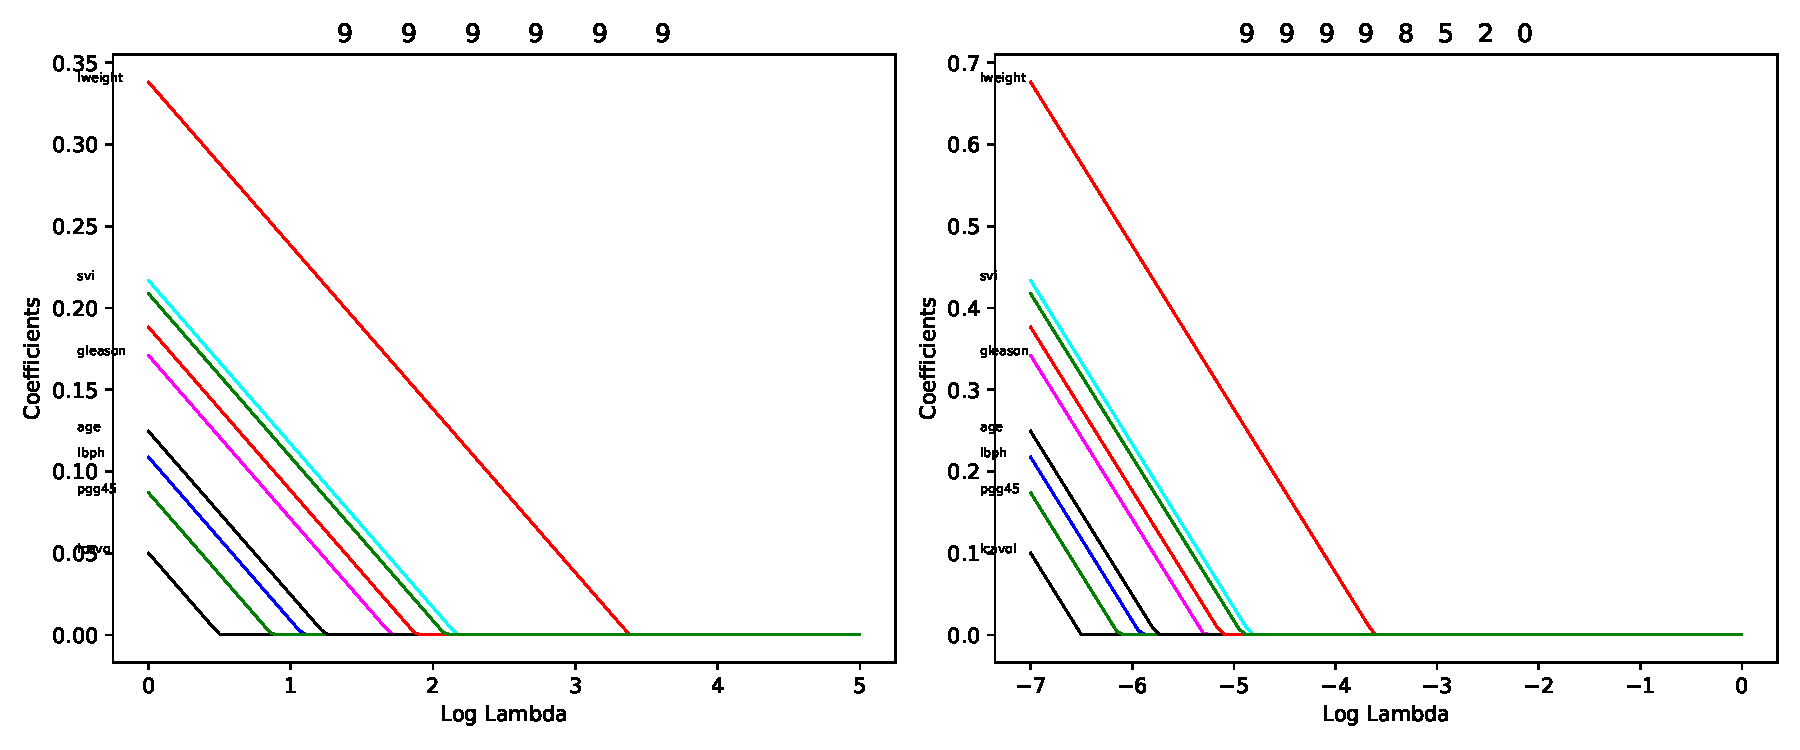
\includegraphics[width=\textwidth]{images/lasso_coef_paths.pdf}
    \caption{Profils des coefficients Lasso en fonction du logarithme de $\lambda$. Contrairement à Ridge, les chemins s'annulent exactement à partir d'un certain seuil de pénalité.}
    \label{fig:lasso_coef_paths}
\end{figure}

\subsection{Propriété de Sélection de Variables (Géométrie)}

Le Lasso peut s'écrire sous forme contrainte :
$$\hat{\beta}^{Lasso} = \arg\min_{\beta \in \mathbb{R}^p} ||y - X\beta||_2^2 \quad \text{s.c.} \quad ||\beta||_1 \le s$$ 
Contrairement à la géométrie circulaire et lisse de Ridge, la région de contrainte du Lasso a la forme d'un polytope, typiquement un losange (ou diamant en 2D) possédant des "coins" extrêmement anguleux et situés exactement sur les axes des coefficients. 
Lorsque les ellipses de contours du RSS s'étendent pour rencontrer cette région de contrainte, la probabilité est extrêmement forte que le premier point de contact "s'accroche" précisément sur l'un de ces coins tranchants (par exemple là où $\beta_1=0$). \textbf{($\bigstar$ EXAMEN)} Cela explique la propriété fondamentale du Lasso : forcer strictement une fraction des coefficients à s'annuler, produisant ainsi des modèles rares (parcimonieux) et agissant mécaniquement comme un opérateur de sélection naturelle de variables.

\begin{figure}[h]
    \centering
    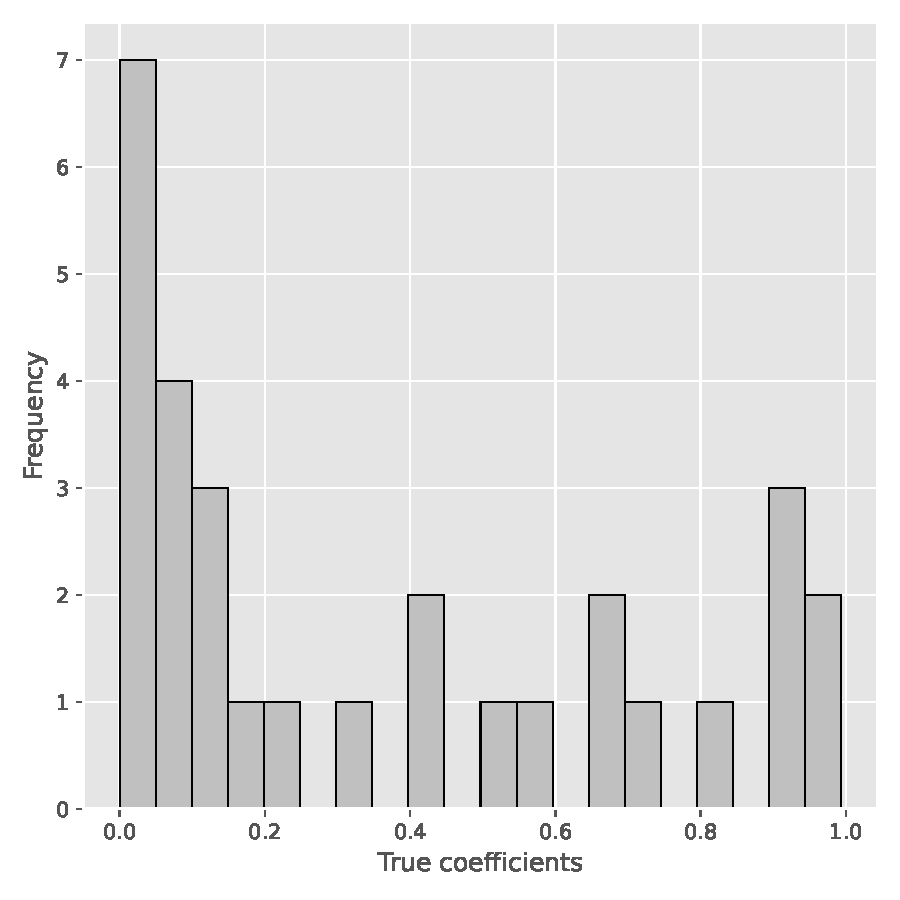
\includegraphics[width=0.45\textwidth]{images/lasso_hist.pdf}
    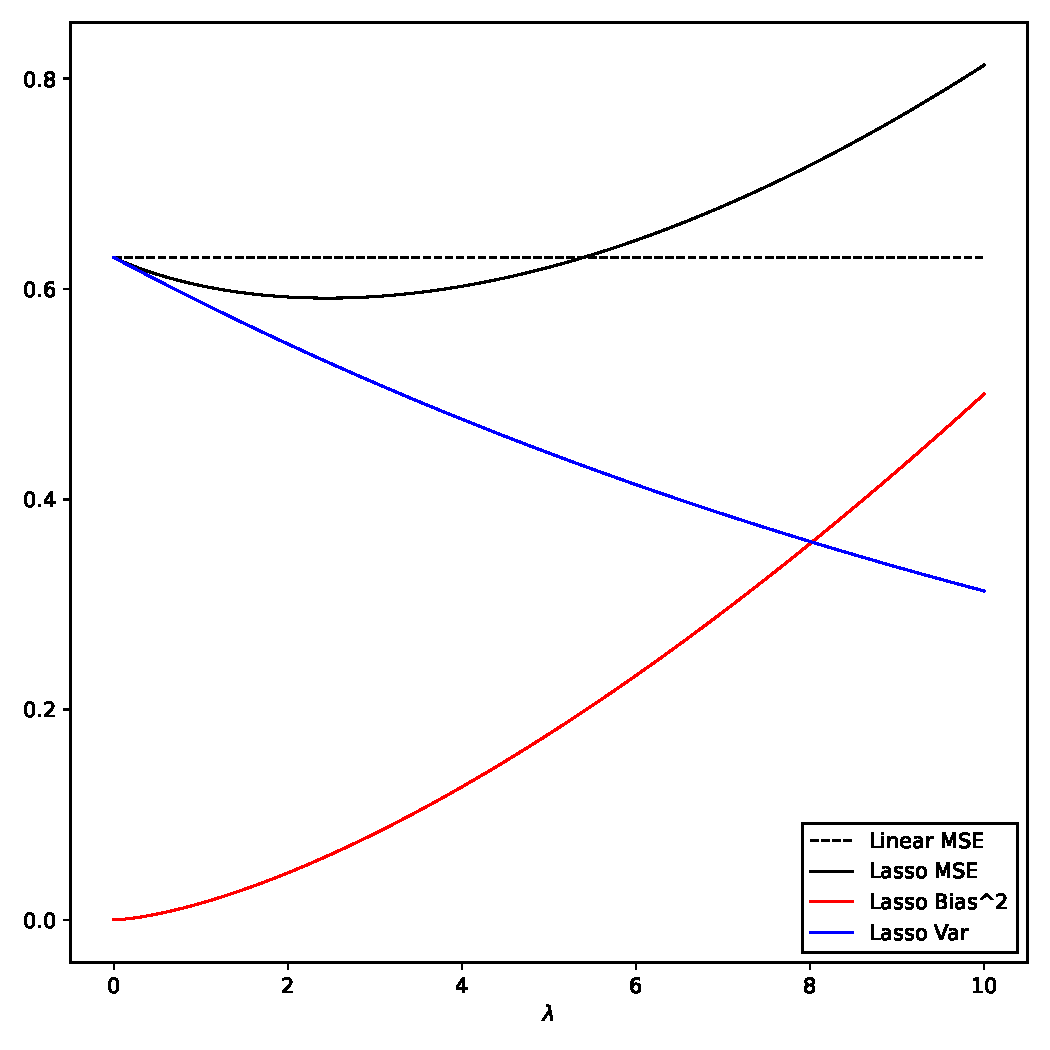
\includegraphics[width=0.5\textwidth]{images/lasso_mse_decomposition.pdf}
    \caption{À gauche: Distribution typique des coefficients sparsifiés par Lasso. À droite: Décomposition du MSE équivalente à celle de Ridge.}
    \label{fig:lasso_hist}
\end{figure}

\subsection{Variantes du LASSO}
Afin de contourner certaines limitations du Lasso standard (par exemple sa difficulté à sélectionner plus de $n$ variables lorsque $p > n$, ou son caractère arbitraire lorsqu'il doit choisir une seule variable parmi un groupe de variables fortement corrélées), plusieurs extensions ont été développées :
\begin{itemize}
    \item \textbf{($\bigstar$ EXAMEN) Elastic Net} : Modèle très populaire qui combine les pénalités $L_1$ (Lasso) et $L_2$ (Ridge). Il minimise $RSS + \lambda_1 \sum |\beta_j| + \lambda_2 \sum \beta_j^2$. L'Elastic Net conserve l'effet de sélection (sparsité) du Lasso tout en bénéficiant de l'effet de groupe (grouping effect) du Ridge pour retenir ensemble des variables corrélées. Il est aussi applicable quand $p > n$.
    \item \textbf{Autres Variantes (Vocabulaire) :} 
    \begin{itemize}
        \item \textit{Fused Lasso} : Pour les données ayant un ordre naturel (ex: séries temporelles), pénalise aussi la différence entre coefficients successifs.
        \item \textit{Grouped Lasso} : Sélectionne ou élimine des groupes entiers de variables (pratique pour les variables catégorielles encodées en multiples *dummies*).
        \item \textit{Adaptive Lasso} : Modifie les poids de pénalité selon l'importance de chaque variable pour garantir que l'estimateur soit un "oracle".
    \end{itemize}
\end{itemize}

\subsection{Implémentation R (glmnet)}
Le package \texttt{glmnet} permet de fiter Ridge (alpha=0) et Lasso (alpha=1). 
La sélection de la valeur optimale de $\lambda$ se fait via validation croisée avec la fonction \texttt{cv.glmnet}.

\begin{verbatim}
library(glmnet)
# x est la matrice des prédicteurs standardisés, y est la réponse
grid <- 10^seq(10, -2, length=100)
# Pour Ridge: alpha=0. (Pour Lasso ce serait alpha=1)
mod.ridge <- glmnet(x, y, alpha=0, lambda=grid)
cv.out <- cv.glmnet(x[train,], y[train], alpha=0)
lambda.cv <- cv.out$lambda.min
\end{verbatim} 

\subsection{Variantes du Lasso}
Pour pallier certaines limites du Lasso (comme l'incapacité de sélectionner plus de $n$ variables quand $p > n$, ou la sélection d'une seule variable au sein d'un groupe très corrélé) , plusieurs variantes ont été développées:
\begin{itemize}
    \item \textbf{Elastic Net} (Zou and Hastie, 2005) : combine les pénalités $L_1$ et $L_2$.
    $$\hat{\beta}^{elnet} = \arg\min_{\beta \in \mathbb{R}^p} ||y - X\beta||_2^2 + \lambda_1||\beta||_1 + \lambda_2||\beta||_2^2$$ 
    \item \textbf{Fused Lasso} (Tibshirani et al., 2005).
    \item \textbf{Adaptive Lasso} (Zou, 2006).
    \item \textbf{Grouped Lasso} (Yuan and Lin, 2007).
\end{itemize}
